%!TEX root = Slic3r-Manual.tex

\section{Sortie SVG} % (fold)
\label{sec:svg_output}
\index{SVG}
\index{DLP resin printer}
\index{imprimante résine DLP}
\index{powder-bed printer}
\index{imprimante à poudre}

Slic3r peut produire une sortie pour d'autres types d'imprimantes 3D qui nécessitent que chaque couche soit représenté en image, par exemple les imprimante résine DLP ou à poudre-lit. Ces imprimantes attendent une image généralement constitué d'une silhouette blanche sur un fond noir (voir figure \ref{fig:example_svg_slice}).  Presque tous les formats d'image peuvent être utilisés (bmp, png, etc), cependant, parce que l'image peut être réduite, il est généralement souhaitable d'utiliser un format vectoriel, plutôt qu'un format bitmap. Pour cette raison, il est courant d'utiliser Scalable Vector Graphics (SVG) format.

\begin{figure}[H]
\centering
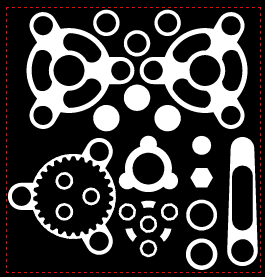
\includegraphics[keepaspectratio=true,width=0.5\textwidth]{advanced/svg_output/example_svg_slice.png}
\caption{Example de tranche SVG.}
\label{fig:example_svg_slice}
\end{figure}

\index{Menu!Slice to SVG...}

Slic3r offre la possibilité de produire une sortie SVG approprié pour de telles imprimantes.  Au lieu d'utiliser le \texttt{Plater}, le processus commence par la sélection de l'option \texttt{Slice to SVG...} du menu \texttt{File}.  Celui-ci demande le fichier source (STL, OBJ ou AMF), et lorsqu'il est sélectionné demande où le fichier SVG de sortie doit être enregistré. Ensuite Slic3r démarre et produit le fichier SVG.

Tenter de voir le fichier SVG dans un navigateur entraînera seulement l'affichage de la première couche, et seules les îles négatifs dans le modèle (comme l'arrière-plan du navigateur est généralement blanc).

\begin{figure}[H]
\centering
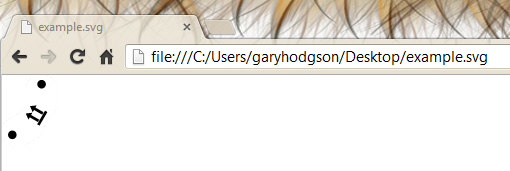
\includegraphics[keepaspectratio=true,width=0.75\textwidth]{advanced/svg_output/svg_direct_browser.png}
\caption{le fichier SVG vu dans un navigateur.}
\label{fig:svg_direct_browser}
\end{figure}

Pour cette raison, une petite application web a été écrite pour permettre de visualiser chaque tranche sur un fond noir\footnote{\url{http://garyhodgson.github.io/slic3rsvgviewer}}.  Accédez à l'application et faites glisser le fichier SVG sur l'écran pour le charger et l'afficher.

\begin{figure}[H]
\centering
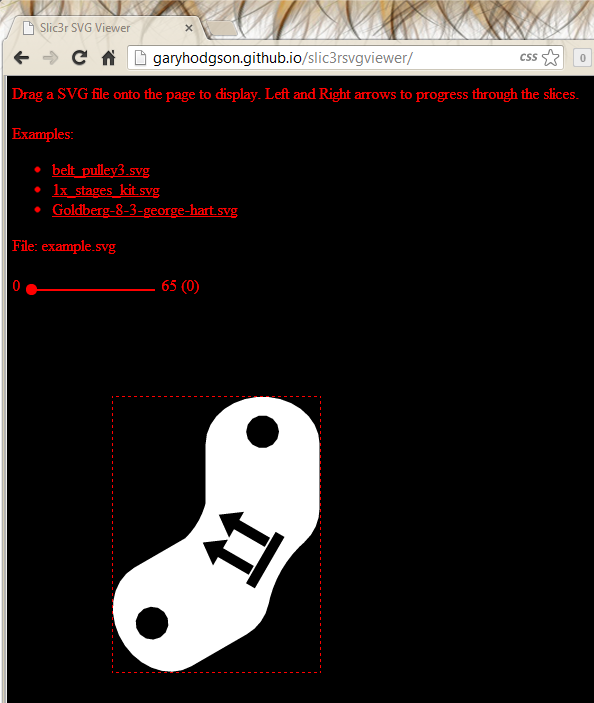
\includegraphics[keepaspectratio=true,width=0.75\textwidth]{advanced/svg_output/svg_slic3rsvg_viewer.png}
\caption{Slic3r SVG Viewer.}
\label{fig:svg_slic3rsvg_viewer}
\end{figure}

\subsection{Paramètres SVG} % (fold)
\label{sub:svg_settings}

La majorité des options dans Slic3r ne sont pas nécessaires pour la génération SVG, cependant le paramètre \texttt{Layer height} déterminera le nombre de couches. Notez que Slic3r limite la hauteur de la couche pour qu'elle soit plus petite que le diamètre de la buse, donc cela peut également être augmenter si l'on souhaite des couches plus hautes.

% subsection svg_settings (end)

\subsection{Imprimer à partir de fichiers SVG} % (fold)
\label{sub:printing_with_svg}

Alors que la sortie SVG peut être utilisé pour une gamme d'imprimantes, l'exemple suivant montre comment le fichier, peut être utilisé avec une imprimante résine DLP. En utilisant une version modifiée de Printrun \footnote{\url{http://garyhodgson.com/reprap/projectlayer}} le fichier SVG peut être chargé directement et envoyé à un projecteur DLP. L'axe Z est contrôlée par des commandes G-code envoyé par le composant printcore, ce qui signifie que l'électronique RepRap standard, tels que RAMPS, peuvent être utilisés.


\begin{figure}[H]
\centering
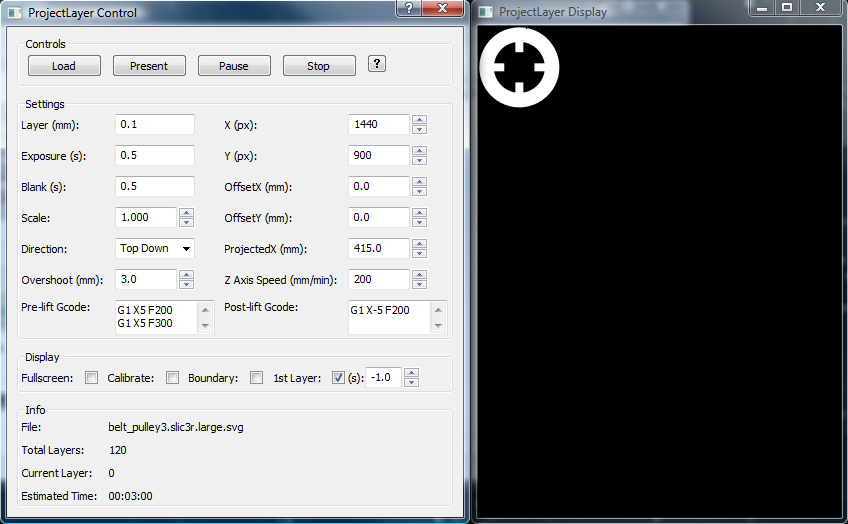
\includegraphics[keepaspectratio=true,width=0.75\textwidth]{advanced/svg_output/projectlayer.png}
\caption{Impression SVG avec Projectlayer.}
\label{fig:projectlayer}
\end{figure}


% subsection printing_with_svg (end)

% section svg_output (end)